\documentclass[11pt,english]{article}
\usepackage[T1]{fontenc}
\usepackage{babel}
\usepackage{textcomp}
\usepackage{graphicx}
\usepackage{float}

\begin{document}

% Define document title and author
\title{Modeling Object Behavior Near Black Holes}
\author{
  Carl Cortright\\
  \texttt{SID: 104731007 Recitation Number: 212 Section Number: 130}
  \and
  Samuel Coyle\\
  \texttt{SID: 105477414 Recitation Number: 243 Section Number: 140}
  \and
  Nelson Botsford\\
  \texttt{SID: 103627718 Recitation Number: 243 Section Number 140}
}
\maketitle

\section*{Introduction}

The study of black holes has classically been restricted to the field of theoretical physics, but lately with movies like Interstellar and Gravity the science has begun to capture the public imagination. While it is impossible to model the inner workings of a black hole beyond the event horizon, we can use differential equations to model the paths of object moving near a black hole, including their relativistic properties. In this report, we analyze the path of an astronaut (Matthew McConaughey) as he descends towards the event horizon from our perspective on a ship whose mission is to seed humanity\textquotesingle s new home planet. Before we lost contact, we were able to model the path of the astronaut with the following differential equation.

\begin{center}
$\frac{dx}{dt} = (\frac{1}{x(t)} - 1) \frac{1}{\sqrt{x(t)}}$
\end{center}

\section*{Understanding the Astronaut\textquotesingle s Path}

To better understand the path of the astronaut, we must first classify the differential equation as autonomous, non-linear, homogeneous, and separable. The astronaut\textquotesingle s speed is the derivative of his position, and the equation is autonomous/homogeneous, meaning that his speed is entirely dependent on his proximity from the center of the black hole.

As mentioned earlier, the speed of the astronaut is the time derivative of position, meaning the differential equation given is the speed of the astronaut as he approaches the black hole. If we have the position of the astronaut, then we are also able to measure his velocity, making it trivial to find his initial velocity.

\begin{center}
$x(0) = 2$,  $v_o = (\frac{1}{2} - 1)\frac{1}{\sqrt{2}} = \frac{-1}{2\sqrt{2}} = -\sqrt{2}$
\end{center}

\section*{Analyzing Existence and Uniqueness of Solution Curves}

Before we decide to use our model as a model for the astronaut\textquotesingle s path, we must first verify that it produces sufficiently unique solutions in proximity of where we want to do our analysis. A useful theorem for defining existence and uniqueness of solutions is Picard\textquotesingle s Theorem which states that the derivative is continuous on a specific rectangle and the second partial derivative with respect to the dependent variable is continuous on that same rectangle, then there exists a unique solution within some interval on the rectangle. Using Picard\textquotesingle s, we first need to find the second partial with respect to x:

\begin{center}
  $\frac{\partial v}{\partial x} = \frac{d}{dx} (\frac{1}{x(t)} - 1) \frac{1}{\sqrt{x(t)}} = \frac{3}{2x^\frac{5}{2}} - \frac{1}{2x^\frac{3}{2}}$
\end{center}

Using this derivative, we are able to tell that there will be a unique solution on any rectangle where all values of x are greater than 0. 

\section*{Positions that Result in no Translation}

Using the equation of the velocity of the velocity given we find that there may be positions where the astronaut will stop moving away or towards the event horizon. These two points where the astronaut will be at equilibrium are x=1 and the limit as x approaches infinity. This makes sense because at the event horizon the astronaut will no longer be moving towards it and as the astronaut gets farther and farther the black hole will have diminishing effect on the astronaut. Unfortunately for the astronaut they will never escape the black hole because for any x value greater than one there is a nonzero velocity.

\begin{figure}[H]
  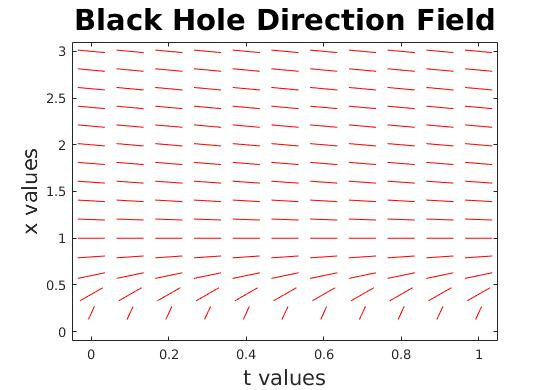
\includegraphics[width=\linewidth]{DirectionField.jpg}
  \caption{The direction field for equation 1.}
  \label{fig:dirfield1}
\end{figure}

\section*{Finding the Path of the Astronaut}

Our most promising option for finding solutions to this differential equation is numerical computation. Analytical solutions are desirable, but in this case it is not worth trying to find one. Instead we can find use various step sizes to compute the following approximations.

\begin{figure}[H]
  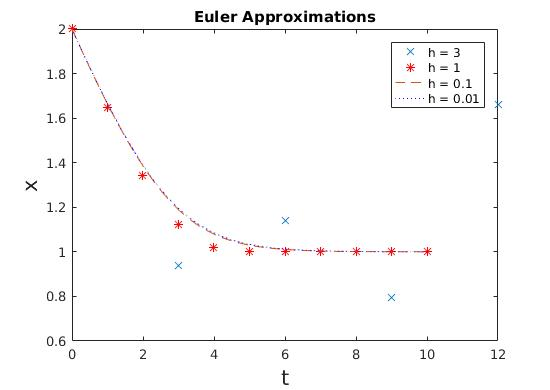
\includegraphics[width=\linewidth]{EulerPlots.jpg}
  \caption{Numerical approximations using Euler\textquotesingle s method starting at x=2.}
  \label{fig:euler1}
\end{figure}

Considering that the plots for step sizes of 0.01 and 0.1are indistinguishable, a step size of 0.1 is enough to give us an accurate approximation without wasting computational resources.

\section*{Long Term Results}

We know that this equation has a unique solution when the starting value of x > 0 as shown in the equation shown below:

\begin{center}
  $\lim_{x\to1} (\frac{1}{x(t)} - 1) \frac{1}{\sqrt{x(t)}} = 0$ 
\end{center}

The limit as t approaches infinity is 0 meaning that from the space station the astronaut will never actually reach the event horizon only approach it. We also know that the long term behavior is independent of the initial condition. This is made clear by the graph shown below.

\begin{figure}[H]
  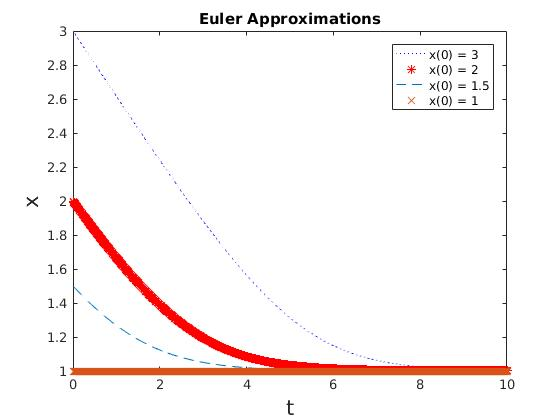
\includegraphics[width=\linewidth]{InitialValuePlots.jpg}
  \caption{Numerical approximations using Euler\textquotesingle s method starting at various different starting points .}
  \label{fig:euler2}
\end{figure}

Regardless of the starting position of the astronaut he will approach an x value of 1. The one exception to this is at a starting position at infinity, where the gravity of the black hole has no effect on him. Both our direction field analysis and our analysis of numerical solutions of this equation agree that our astronaut will approach the event horizon asymptotically.

\section*{Conclusion}

Our astronaut will never reach the event horizon of the black hole, at least from the perspective of observers on the space station. Instead he will approach it, quickly at first, but he will soon slow down and be doomed to spend an eternity gravitating towards the event horizon. 

% Your document ends here!
\end{document}
